% Options for packages loaded elsewhere
\PassOptionsToPackage{unicode}{hyperref}
\PassOptionsToPackage{hyphens}{url}
%
\documentclass[
]{article}
\usepackage{amsmath,amssymb}
\usepackage{iftex}
\ifPDFTeX
  \usepackage[T1]{fontenc}
  \usepackage[utf8]{inputenc}
  \usepackage{textcomp} % provide euro and other symbols
\else % if luatex or xetex
  \usepackage{unicode-math} % this also loads fontspec
  \defaultfontfeatures{Scale=MatchLowercase}
  \defaultfontfeatures[\rmfamily]{Ligatures=TeX,Scale=1}
\fi
\usepackage{lmodern}
\ifPDFTeX\else
  % xetex/luatex font selection
\fi
% Use upquote if available, for straight quotes in verbatim environments
\IfFileExists{upquote.sty}{\usepackage{upquote}}{}
\IfFileExists{microtype.sty}{% use microtype if available
  \usepackage[]{microtype}
  \UseMicrotypeSet[protrusion]{basicmath} % disable protrusion for tt fonts
}{}
\makeatletter
\@ifundefined{KOMAClassName}{% if non-KOMA class
  \IfFileExists{parskip.sty}{%
    \usepackage{parskip}
  }{% else
    \setlength{\parindent}{0pt}
    \setlength{\parskip}{6pt plus 2pt minus 1pt}}
}{% if KOMA class
  \KOMAoptions{parskip=half}}
\makeatother
\usepackage{xcolor}
\usepackage[margin=1in]{geometry}
\usepackage{color}
\usepackage{fancyvrb}
\newcommand{\VerbBar}{|}
\newcommand{\VERB}{\Verb[commandchars=\\\{\}]}
\DefineVerbatimEnvironment{Highlighting}{Verbatim}{commandchars=\\\{\}}
% Add ',fontsize=\small' for more characters per line
\usepackage{framed}
\definecolor{shadecolor}{RGB}{248,248,248}
\newenvironment{Shaded}{\begin{snugshade}}{\end{snugshade}}
\newcommand{\AlertTok}[1]{\textcolor[rgb]{0.94,0.16,0.16}{#1}}
\newcommand{\AnnotationTok}[1]{\textcolor[rgb]{0.56,0.35,0.01}{\textbf{\textit{#1}}}}
\newcommand{\AttributeTok}[1]{\textcolor[rgb]{0.13,0.29,0.53}{#1}}
\newcommand{\BaseNTok}[1]{\textcolor[rgb]{0.00,0.00,0.81}{#1}}
\newcommand{\BuiltInTok}[1]{#1}
\newcommand{\CharTok}[1]{\textcolor[rgb]{0.31,0.60,0.02}{#1}}
\newcommand{\CommentTok}[1]{\textcolor[rgb]{0.56,0.35,0.01}{\textit{#1}}}
\newcommand{\CommentVarTok}[1]{\textcolor[rgb]{0.56,0.35,0.01}{\textbf{\textit{#1}}}}
\newcommand{\ConstantTok}[1]{\textcolor[rgb]{0.56,0.35,0.01}{#1}}
\newcommand{\ControlFlowTok}[1]{\textcolor[rgb]{0.13,0.29,0.53}{\textbf{#1}}}
\newcommand{\DataTypeTok}[1]{\textcolor[rgb]{0.13,0.29,0.53}{#1}}
\newcommand{\DecValTok}[1]{\textcolor[rgb]{0.00,0.00,0.81}{#1}}
\newcommand{\DocumentationTok}[1]{\textcolor[rgb]{0.56,0.35,0.01}{\textbf{\textit{#1}}}}
\newcommand{\ErrorTok}[1]{\textcolor[rgb]{0.64,0.00,0.00}{\textbf{#1}}}
\newcommand{\ExtensionTok}[1]{#1}
\newcommand{\FloatTok}[1]{\textcolor[rgb]{0.00,0.00,0.81}{#1}}
\newcommand{\FunctionTok}[1]{\textcolor[rgb]{0.13,0.29,0.53}{\textbf{#1}}}
\newcommand{\ImportTok}[1]{#1}
\newcommand{\InformationTok}[1]{\textcolor[rgb]{0.56,0.35,0.01}{\textbf{\textit{#1}}}}
\newcommand{\KeywordTok}[1]{\textcolor[rgb]{0.13,0.29,0.53}{\textbf{#1}}}
\newcommand{\NormalTok}[1]{#1}
\newcommand{\OperatorTok}[1]{\textcolor[rgb]{0.81,0.36,0.00}{\textbf{#1}}}
\newcommand{\OtherTok}[1]{\textcolor[rgb]{0.56,0.35,0.01}{#1}}
\newcommand{\PreprocessorTok}[1]{\textcolor[rgb]{0.56,0.35,0.01}{\textit{#1}}}
\newcommand{\RegionMarkerTok}[1]{#1}
\newcommand{\SpecialCharTok}[1]{\textcolor[rgb]{0.81,0.36,0.00}{\textbf{#1}}}
\newcommand{\SpecialStringTok}[1]{\textcolor[rgb]{0.31,0.60,0.02}{#1}}
\newcommand{\StringTok}[1]{\textcolor[rgb]{0.31,0.60,0.02}{#1}}
\newcommand{\VariableTok}[1]{\textcolor[rgb]{0.00,0.00,0.00}{#1}}
\newcommand{\VerbatimStringTok}[1]{\textcolor[rgb]{0.31,0.60,0.02}{#1}}
\newcommand{\WarningTok}[1]{\textcolor[rgb]{0.56,0.35,0.01}{\textbf{\textit{#1}}}}
\usepackage{graphicx}
\makeatletter
\def\maxwidth{\ifdim\Gin@nat@width>\linewidth\linewidth\else\Gin@nat@width\fi}
\def\maxheight{\ifdim\Gin@nat@height>\textheight\textheight\else\Gin@nat@height\fi}
\makeatother
% Scale images if necessary, so that they will not overflow the page
% margins by default, and it is still possible to overwrite the defaults
% using explicit options in \includegraphics[width, height, ...]{}
\setkeys{Gin}{width=\maxwidth,height=\maxheight,keepaspectratio}
% Set default figure placement to htbp
\makeatletter
\def\fps@figure{htbp}
\makeatother
\setlength{\emergencystretch}{3em} % prevent overfull lines
\providecommand{\tightlist}{%
  \setlength{\itemsep}{0pt}\setlength{\parskip}{0pt}}
\setcounter{secnumdepth}{-\maxdimen} % remove section numbering
\ifLuaTeX
  \usepackage{selnolig}  % disable illegal ligatures
\fi
\usepackage{bookmark}
\IfFileExists{xurl.sty}{\usepackage{xurl}}{} % add URL line breaks if available
\urlstyle{same}
\hypersetup{
  hidelinks,
  pdfcreator={LaTeX via pandoc}}

\author{}
\date{\vspace{-2.5em}}

\begin{document}

Stacy Chen title: ``Project 8 Template'' output: pdf\_document ---

\begin{Shaded}
\begin{Highlighting}[]
\CommentTok{\# Add to this package list for additional SL algorithms}
\NormalTok{pacman}\SpecialCharTok{::}\FunctionTok{p\_load}\NormalTok{(}
\NormalTok{  tidyverse,}
\NormalTok{  ggthemes,}
\NormalTok{  ltmle,}
\NormalTok{  tmle,}
\NormalTok{  SuperLearner,}
\NormalTok{  tidymodels,}
\NormalTok{  caret,}
\NormalTok{  dagitty,}
\NormalTok{  ggdag,}
\NormalTok{  here)}

\NormalTok{heart\_disease }\OtherTok{\textless{}{-}} \FunctionTok{read\_csv}\NormalTok{(}\FunctionTok{here}\NormalTok{(}\StringTok{\textquotesingle{}/Users/stacyworkuser/Downloads/heart\_disease\_tmle.csv\textquotesingle{}}\NormalTok{))}
\end{Highlighting}
\end{Shaded}

\begin{verbatim}
## Rows: 10000 Columns: 14
## -- Column specification --------------------------------------------------------
## Delimiter: ","
## dbl (14): age, sex_at_birth, simplified_race, college_educ, income_thousands...
## 
## i Use `spec()` to retrieve the full column specification for this data.
## i Specify the column types or set `show_col_types = FALSE` to quiet this message.
\end{verbatim}

\section{Introduction}\label{introduction}

Heart disease is the leading cause of death in the United States, and
treating it properly is an important public health goal. However, it is
a complex disease with several different risk factors and potential
treatments. Physicians typically recommend changes in diet, increased
exercise, and/or medication to treat symptoms, but it is difficult to
determine how effective any one of these factors is in treating the
disease. In this project, you will explore SuperLearner, Targeted
Maximum Likelihood Estimation (TMLE), and Longitudinal Targeted Maximum
Likelihood Estimation (LTMLE). Using a simulated dataset, you will
explore whether taking blood pressure medication reduces mortality risk.

\section{Data}\label{data}

This dataset was simulated using R (so it does not come from a previous
study or other data source). It contains several variables:

\section{SuperLearner}\label{superlearner}

\subsection{Modeling}\label{modeling}

\begin{Shaded}
\begin{Highlighting}[]
\NormalTok{train\_index }\OtherTok{\textless{}{-}} \FunctionTok{createDataPartition}\NormalTok{(heart\_disease}\SpecialCharTok{$}\NormalTok{mortality, }\AttributeTok{p =} \FloatTok{0.75}\NormalTok{, }\AttributeTok{list =} \ConstantTok{FALSE}\NormalTok{) }\CommentTok{\#mortality outcome variable }
\NormalTok{train\_data }\OtherTok{\textless{}{-}}\NormalTok{ heart\_disease[train\_index, ]}
\NormalTok{test\_data }\OtherTok{\textless{}{-}}\NormalTok{ heart\_disease[}\SpecialCharTok{{-}}\NormalTok{train\_index, ]}

\DocumentationTok{\#\# sl libraries}
\NormalTok{sl\_lib }\OtherTok{\textless{}{-}} \FunctionTok{c}\NormalTok{(}\StringTok{"SL.nnet"}\NormalTok{, }\StringTok{"SL.glmnet"}\NormalTok{, }\StringTok{"SL.randomForest"}\NormalTok{, }\StringTok{"SL.glm"}\NormalTok{, }\StringTok{"SL.lm"}\NormalTok{)}

\NormalTok{sl }\OtherTok{=} \FunctionTok{SuperLearner}\NormalTok{(}\AttributeTok{Y =}\NormalTok{ train\_data}\SpecialCharTok{$}\NormalTok{mortality,}
                  \AttributeTok{X =}\NormalTok{ train\_data }\SpecialCharTok{\%\textgreater{}\%}
                                        \FunctionTok{select}\NormalTok{(age, sex\_at\_birth, simplified\_race, college\_educ, income\_thousands, blood\_pressure, chol, blood\_pressure\_medication, bmi),}
                  \AttributeTok{family =} \FunctionTok{binomial}\NormalTok{(),}
                  \AttributeTok{SL.library =}\NormalTok{ sl\_lib)}
\end{Highlighting}
\end{Shaded}

\begin{verbatim}
## Loading required namespace: randomForest
\end{verbatim}

\begin{Shaded}
\begin{Highlighting}[]
\NormalTok{coefficients }\OtherTok{\textless{}{-}}\NormalTok{ sl}\SpecialCharTok{$}\NormalTok{coef}
\NormalTok{risks }\OtherTok{\textless{}{-}}\NormalTok{ sl}\SpecialCharTok{$}\NormalTok{coef}

\FunctionTok{print}\NormalTok{(coefficients)}
\end{Highlighting}
\end{Shaded}

\begin{verbatim}
##         SL.nnet_All       SL.glmnet_All SL.randomForest_All          SL.glm_All 
##          0.03443923          0.00000000          0.60132789          0.00000000 
##           SL.lm_All 
##          0.36423288
\end{verbatim}

\begin{Shaded}
\begin{Highlighting}[]
\FunctionTok{print}\NormalTok{(risks)}
\end{Highlighting}
\end{Shaded}

\begin{verbatim}
##         SL.nnet_All       SL.glmnet_All SL.randomForest_All          SL.glm_All 
##          0.03443923          0.00000000          0.60132789          0.00000000 
##           SL.lm_All 
##          0.36423288
\end{verbatim}

\begin{Shaded}
\begin{Highlighting}[]
\CommentTok{\#discrete winner}
\NormalTok{sl}\SpecialCharTok{$}\NormalTok{cvRisk[}\FunctionTok{which.min}\NormalTok{(sl}\SpecialCharTok{$}\NormalTok{cvRisk)]}
\end{Highlighting}
\end{Shaded}

\begin{verbatim}
## SL.randomForest_All 
##           0.2326556
\end{verbatim}

\begin{Shaded}
\begin{Highlighting}[]
\NormalTok{sl}\SpecialCharTok{$}\NormalTok{coef[}\FunctionTok{which.min}\NormalTok{(sl}\SpecialCharTok{$}\NormalTok{coef)]}
\end{Highlighting}
\end{Shaded}

\begin{verbatim}
## SL.glmnet_All 
##             0
\end{verbatim}

\begin{Shaded}
\begin{Highlighting}[]
\CommentTok{\# getting predictions and reporting confusion matrix}
\NormalTok{predictions }\OtherTok{\textless{}{-}} \FunctionTok{predict}\NormalTok{(sl, }\AttributeTok{newdata =}\NormalTok{ test\_data }\SpecialCharTok{\%\textgreater{}\%} 
                        \FunctionTok{select}\NormalTok{(age, sex\_at\_birth, simplified\_race, college\_educ, income\_thousands, blood\_pressure, chol, blood\_pressure\_medication, bmi), }\AttributeTok{type =} \StringTok{"response"}\NormalTok{)}

\NormalTok{predicted\_class }\OtherTok{\textless{}{-}} \FunctionTok{ifelse}\NormalTok{(predictions}\SpecialCharTok{$}\NormalTok{pred }\SpecialCharTok{\textgreater{}=} \FloatTok{0.5}\NormalTok{, }\DecValTok{1}\NormalTok{, }\DecValTok{0}\NormalTok{)}
\NormalTok{conf\_matrix }\OtherTok{\textless{}{-}} \FunctionTok{table}\NormalTok{(}\AttributeTok{Predicted =}\NormalTok{ predicted\_class, }\AttributeTok{Actual =}\NormalTok{ test\_data}\SpecialCharTok{$}\NormalTok{mortality)}
\FunctionTok{confusionMatrix}\NormalTok{(conf\_matrix)}
\end{Highlighting}
\end{Shaded}

\begin{verbatim}
## Confusion Matrix and Statistics
## 
##          Actual
## Predicted    0    1
##         0  414  246
##         1  765 1075
##                                           
##                Accuracy : 0.5956          
##                  95% CI : (0.5761, 0.6149)
##     No Information Rate : 0.5284          
##     P-Value [Acc > NIR] : 8.045e-12       
##                                           
##                   Kappa : 0.1689          
##                                           
##  Mcnemar's Test P-Value : < 2.2e-16       
##                                           
##             Sensitivity : 0.3511          
##             Specificity : 0.8138          
##          Pos Pred Value : 0.6273          
##          Neg Pred Value : 0.5842          
##              Prevalence : 0.4716          
##          Detection Rate : 0.1656          
##    Detection Prevalence : 0.2640          
##       Balanced Accuracy : 0.5825          
##                                           
##        'Positive' Class : 0               
## 
\end{verbatim}

\begin{Shaded}
\begin{Highlighting}[]
\CommentTok{\# Accuracy, Recall, and Precision}
\NormalTok{accuracy }\OtherTok{\textless{}{-}} \FunctionTok{sum}\NormalTok{(}\FunctionTok{diag}\NormalTok{(conf\_matrix)) }\SpecialCharTok{/} \FunctionTok{sum}\NormalTok{(conf\_matrix)}
\NormalTok{recall }\OtherTok{\textless{}{-}}\NormalTok{ conf\_matrix[}\DecValTok{2}\NormalTok{, }\DecValTok{2}\NormalTok{] }\SpecialCharTok{/} \FunctionTok{sum}\NormalTok{(conf\_matrix[}\DecValTok{2}\NormalTok{, ])}
\NormalTok{precision }\OtherTok{\textless{}{-}}\NormalTok{ conf\_matrix[}\DecValTok{2}\NormalTok{, }\DecValTok{2}\NormalTok{] }\SpecialCharTok{/} \FunctionTok{sum}\NormalTok{(conf\_matrix[, }\DecValTok{2}\NormalTok{])}
\FunctionTok{list}\NormalTok{(}\AttributeTok{Accuracy =}\NormalTok{ accuracy, }\AttributeTok{Recall =}\NormalTok{ recall, }\AttributeTok{Precision =}\NormalTok{ precision)}
\end{Highlighting}
\end{Shaded}

\begin{verbatim}
## $Accuracy
## [1] 0.5956
## 
## $Recall
## [1] 0.5842391
## 
## $Precision
## [1] 0.8137774
\end{verbatim}

\subsection{Discussion Questions}\label{discussion-questions}

Why should we, in general, prefer the SuperLearner ensemble to the
discrete winner in cross-validation? Or in other words, what is the
advantage of ``blending'' algorithms together and giving them each
weights, rather than just using the single best algorithm (with best
being defined as minimizing risk)?

*Answer: With multiple algorithms, each one can take better advantage of
strengths of the algorithm to improve prediction. It can also be more
robust to new data and generalize better to data with different
distribution instead of overfitting. It also helps mitigate the impact
of outliers in data and reduces variance and bias.

\section{Targeted Maximum Likelihood
Estimation}\label{targeted-maximum-likelihood-estimation}

\subsection{Causal Diagram}\label{causal-diagram}

TMLE requires estimating two models:

Using ggdag and daggity, draw a directed acylcic graph (DAG) that
describes the relationships between the outcome, treatment, and
covariates/predictors. Note, if you think there are covariates that are
not related to other variables in the dataset, note this by either
including them as freestanding nodes or by omitting them and noting
omissions in your discussion.

\begin{Shaded}
\begin{Highlighting}[]
\NormalTok{tmle\_dag}\OtherTok{\textless{}{-}}\FunctionTok{dagify}\NormalTok{(medication }\SpecialCharTok{\textasciitilde{}}\NormalTok{ race }\SpecialCharTok{+}\NormalTok{ college\_edc }\SpecialCharTok{+}\NormalTok{ chol }\SpecialCharTok{+}\NormalTok{ bmi}\SpecialCharTok{+}\NormalTok{ income }\SpecialCharTok{+}\NormalTok{ blood\_pressure }\SpecialCharTok{+}\NormalTok{ unobserved\_factors,}
\NormalTok{                 mortality }\SpecialCharTok{\textasciitilde{}}\NormalTok{ medication }\SpecialCharTok{+}\NormalTok{ age }\SpecialCharTok{+}\NormalTok{ race }\SpecialCharTok{+}\NormalTok{ sex }\SpecialCharTok{+}\NormalTok{ unobserved\_factors,}
                 \AttributeTok{exposure =} \StringTok{"medication"}\NormalTok{,}
                 \AttributeTok{outcome=}\StringTok{"mortality"}
\NormalTok{)}

\FunctionTok{ggdag}\NormalTok{(tmle\_dag)}
\end{Highlighting}
\end{Shaded}

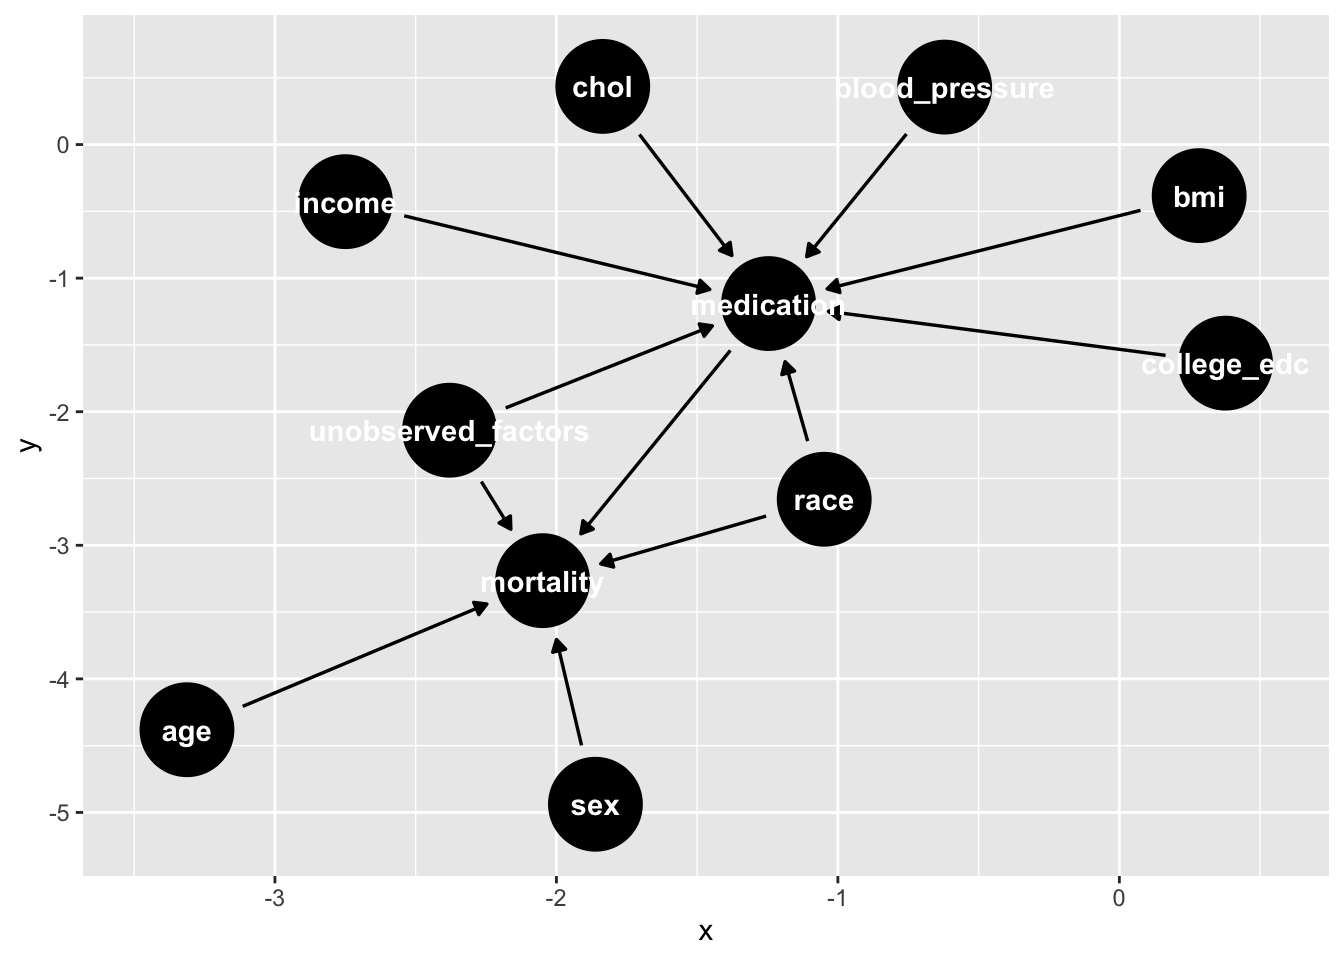
\includegraphics{Project-8-SC_files/figure-latex/unnamed-chunk-5-1.pdf}

\subsection{TMLE Estimation}\label{tmle-estimation}

Use the \texttt{tmle} package to estimate a model for the effect of
blood pressure medication on the probability of mortality. Do the
following:

\begin{Shaded}
\begin{Highlighting}[]
\NormalTok{Y}\OtherTok{\textless{}{-}}\NormalTok{heart\_disease}\SpecialCharTok{$}\NormalTok{mortality}
\NormalTok{A}\OtherTok{\textless{}{-}}\NormalTok{heart\_disease}\SpecialCharTok{$}\NormalTok{blood\_pressure\_medication}
\NormalTok{W}\OtherTok{\textless{}{-}}\NormalTok{heart\_disease}\SpecialCharTok{\%\textgreater{}\%}\FunctionTok{select}\NormalTok{(sex\_at\_birth, age, simplified\_race)}

\NormalTok{tmle\_result }\OtherTok{\textless{}{-}} \FunctionTok{tmle}\NormalTok{(}\AttributeTok{Y=}\NormalTok{Y,}
                    \AttributeTok{A=}\NormalTok{A,}
                    \AttributeTok{W=}\NormalTok{W,}
                    \AttributeTok{family=}\StringTok{"binomial"}\NormalTok{,}
                    \AttributeTok{Q.SL.library =}\NormalTok{ sl\_lib,}
                    \AttributeTok{g.SL.library =}\NormalTok{ sl\_lib)}
\FunctionTok{summary}\NormalTok{(tmle\_result)}
\end{Highlighting}
\end{Shaded}

\begin{verbatim}
##  Initial estimation of Q
##   Procedure: cv-SuperLearner, ensemble
##   Model:
##       Y ~  SL.nnet_All + SL.glmnet_All + SL.randomForest_All + SL.glm_All + SL.lm_All
## 
##   Coefficients: 
##       SL.nnet_All    0 
##     SL.glmnet_All    0.9945481 
##   SL.randomForest_All    0.005451915 
##        SL.glm_All    0 
##         SL.lm_All    0 
## 
##   Cross-validated pseudo R squared :  0.0386 
## 
##  Estimation of g (treatment mechanism)
##   Procedure: SuperLearner, ensemble
##   Model:
##       A ~  SL.nnet_All + SL.glmnet_All + SL.randomForest_All + SL.glm_All + SL.lm_All 
## 
##   Coefficients: 
##       SL.nnet_All    0.06370584 
##     SL.glmnet_All    0.3876352 
##   SL.randomForest_All    0 
##        SL.glm_All    0 
##         SL.lm_All    0.548659 
## 
##  Estimation of g.Z (intermediate variable assignment mechanism)
##   Procedure: No intermediate variable 
## 
##  Estimation of g.Delta (missingness mechanism)
##   Procedure: No missingness, ensemble
## 
##  Bounds on g: (0.0054, 1) 
## 
##  Bounds on g for ATT/ATC: (0.0054, 0.9946) 
## 
##  Marginal Mean under Treatment (EY1)
##    Parameter Estimate:  0.24886
##    Estimated Variance:  0.00013723
##               p-value:  <2e-16
##     95% Conf Interval:  (0.2259, 0.27182)
## 
##  Marginal Mean under Comparator (EY0)
##    Parameter Estimate:  0.5657
##    Estimated Variance:  2.8417e-05
##               p-value:  <2e-16
##     95% Conf Interval:  (0.55525, 0.57615)
## 
##  Additive Effect
##    Parameter Estimate:  -0.31684
##    Estimated Variance:  0.00016561
##               p-value:  <2e-16
##     95% Conf Interval:  (-0.34206, -0.29161)
## 
##  Additive Effect among the Treated
##    Parameter Estimate:  -0.31551
##    Estimated Variance:  0.00015037
##               p-value:  <2e-16
##     95% Conf Interval:  (-0.33954, -0.29147)
## 
##  Additive Effect among the Controls
##    Parameter Estimate:  -0.31754
##    Estimated Variance:  0.00014938
##               p-value:  <2e-16
##     95% Conf Interval:  (-0.34149, -0.29358)
## 
##  Relative Risk
##    Parameter  Estimate:  0.43992
##    Variance(log scale):  0.0023043
##                p-value:  <2e-16
##      95% Conf Interval:  (0.40042, 0.48332)
## 
##  Odds Ratio
##     Parameter  Estimate:  0.25436
##     Variance(log scale):  0.0043972
##                 p-value:  <2e-16
##       95% Conf Interval:  (0.22336, 0.28966)
\end{verbatim}

\begin{Shaded}
\begin{Highlighting}[]
\NormalTok{tmle\_result}\SpecialCharTok{$}\NormalTok{estimates}\SpecialCharTok{$}\NormalTok{ATE}
\end{Highlighting}
\end{Shaded}

\begin{verbatim}
## $psi
## [1] -0.3168356
## 
## $var.psi
## [1] 0.000165606
## 
## $CI
## [1] -0.3420580 -0.2916132
## 
## $pvalue
## [1] 7.630242e-134
## 
## $bs.var
## [1] NA
## 
## $bs.CI.twosided
## [1] NA NA
## 
## $bs.CI.onesided.lower
## [1] -Inf   NA
## 
## $bs.CI.onesided.upper
## [1]  NA Inf
\end{verbatim}

\subsection{Discussion Questions}\label{discussion-questions-1}

What is a ``double robust'' estimator? Why does it provide a guarantee
of consistency if either the outcome model or propensity score model is
correctly specified? Or in other words, why does mispecifying one of the
models not break the analysis? When answering this question, think about
how your introductory statistics courses emphasized using theory to
determine the correct outcome model, and in this course how we explored
the benefits of matching. Answer: A doubly robust estimator combines two
models to estimate a target parameter. They're consistent even when the
outcome model is misspecified. It is able to do this because the
estimator can leverage different both outcome and propoensity score
estimation approaches and upweight outputs of the correctly specified
approach.

\section{LTMLE Estimation}\label{ltmle-estimation}

\subsection{Causal Diagram}\label{causal-diagram-1}

\begin{Shaded}
\begin{Highlighting}[]
\CommentTok{\# DAG for TMLE{-}reducing complexity by combining covariates (sex, age, college education, income, etc)}
\NormalTok{dag }\OtherTok{\textless{}{-}}\NormalTok{ dagitty}\SpecialCharTok{::}\FunctionTok{dagitty}\NormalTok{(}\StringTok{"}
\StringTok{dag \{}
\StringTok{  unobserved\_factors [unobserved]}
\StringTok{  unobserved\_factors [unobserved]}
\StringTok{  Covariates\_t2{-}\textgreater{} Treatment\_t2 {-}\textgreater{} Mortality}
\StringTok{  Covariates\_t2 {-}\textgreater{} Mortality}
\StringTok{  Covariates\_t1 {-}\textgreater{} Mortality}
\StringTok{   Covariates\_t1 {-}\textgreater{} Treatment\_t1}
\StringTok{  Covariates\_t1 {-}\textgreater{} Treatment\_t2}
\StringTok{  Treatment\_t2 {-}\textgreater{} Mortality}
\StringTok{   Treatment\_t1 {-}\textgreater{} Mortality}
\StringTok{  unobserved\_factors {-}\textgreater{} Covariates\_t1}
\StringTok{  unobserved\_factors {-}\textgreater{} Treatment\_t1}
\StringTok{    unobserved\_factors {-}\textgreater{} Covariates\_t2}
\StringTok{  unobserved\_factors {-}\textgreater{} Treatment\_t2}
\StringTok{\}}
\StringTok{"}\NormalTok{)}


\NormalTok{ggdag }\OtherTok{\textless{}{-}}\NormalTok{ ggdag}\SpecialCharTok{::}\FunctionTok{ggdag}\NormalTok{(dag, }\AttributeTok{text =} \ConstantTok{TRUE}\NormalTok{, }\AttributeTok{use\_labels =} \StringTok{"name"}\NormalTok{, }\AttributeTok{layout =} \StringTok{"circle"}\NormalTok{) }\SpecialCharTok{+}
  \FunctionTok{theme\_minimal}\NormalTok{() }\SpecialCharTok{+}
  \FunctionTok{ggtitle}\NormalTok{(}\StringTok{"Longitudinal DAG"}\NormalTok{)}

\CommentTok{\# Print the DAG}
\FunctionTok{print}\NormalTok{(ggdag)}
\end{Highlighting}
\end{Shaded}

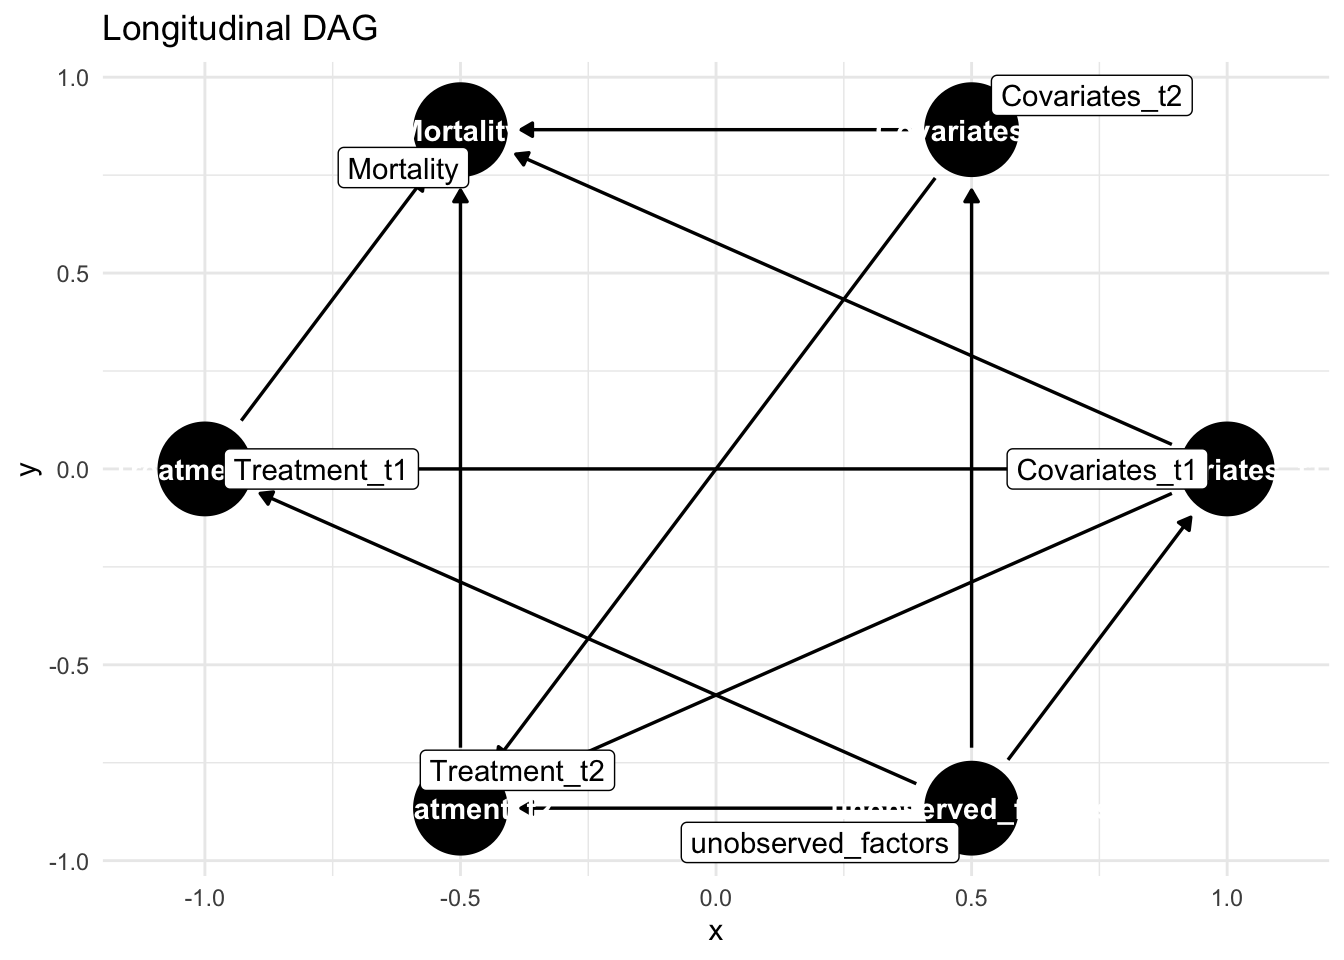
\includegraphics{Project-8-SC_files/figure-latex/unnamed-chunk-7-1.pdf}

\subsection{LTMLE Estimation}\label{ltmle-estimation-1}

\begin{Shaded}
\begin{Highlighting}[]
\CommentTok{\#LTMLE}
\NormalTok{ltmle\_data }\OtherTok{\textless{}{-}}\NormalTok{heart\_disease}\SpecialCharTok{\%\textgreater{}\%}\FunctionTok{select}\NormalTok{(age, simplified\_race, income\_thousands, sex\_at\_birth, chol, bmi, blood\_pressure, blood\_pressure\_medication, bmi\_2, chol\_2, blood\_pressure\_2, blood\_pressure\_medication\_2, mortality)}
\CommentTok{\#define nodes {-} don\textquotesingle{}t think you need to define W because it just assumes whatever is to the left of A1 is W}
\NormalTok{Anodes}\OtherTok{\textless{}{-}}\FunctionTok{c}\NormalTok{(}\StringTok{"blood\_pressure\_medication"}\NormalTok{, }\StringTok{"blood\_pressure\_medication\_2"}\NormalTok{)}
\NormalTok{Ynodes}\OtherTok{\textless{}{-}}\StringTok{"mortality"}
\NormalTok{Lnodes}\OtherTok{\textless{}{-}}\FunctionTok{c}\NormalTok{(}\StringTok{"bmi\_2"}\NormalTok{, }\StringTok{"chol\_2"}\NormalTok{, }\StringTok{"blood\_pressure\_2"}\NormalTok{)}

\DocumentationTok{\#\# Naive Model (no time{-}dependent confounding) estimate}
\NormalTok{ltmle\_naive\_data}\OtherTok{\textless{}{-}}\NormalTok{ltmle\_data}\SpecialCharTok{\%\textgreater{}\%}\FunctionTok{select}\NormalTok{(}\SpecialCharTok{{-}}\NormalTok{bmi\_2, }\SpecialCharTok{{-}}\NormalTok{chol\_2, }\SpecialCharTok{{-}}\NormalTok{blood\_pressure\_2)}
\NormalTok{ltmle\_naive}\OtherTok{\textless{}{-}}\FunctionTok{ltmle}\NormalTok{(ltmle\_naive\_data, }\AttributeTok{Anodes=}\NormalTok{Anodes, }\AttributeTok{Ynodes=}\NormalTok{Ynodes, }\AttributeTok{abar=}\FunctionTok{c}\NormalTok{(}\DecValTok{1}\NormalTok{, }\DecValTok{1}\NormalTok{), }\AttributeTok{SL.library=}\NormalTok{sl\_lib)}
\end{Highlighting}
\end{Shaded}

\begin{verbatim}
## Qform not specified, using defaults:
\end{verbatim}

\begin{verbatim}
## formula for mortality:
\end{verbatim}

\begin{verbatim}
## Q.kplus1 ~ age + simplified_race + income_thousands + sex_at_birth +     chol + bmi + blood_pressure + blood_pressure_medication +     blood_pressure_medication_2
\end{verbatim}

\begin{verbatim}
## 
\end{verbatim}

\begin{verbatim}
## gform not specified, using defaults:
\end{verbatim}

\begin{verbatim}
## formula for blood_pressure_medication:
\end{verbatim}

\begin{verbatim}
## blood_pressure_medication ~ age + simplified_race + income_thousands +     sex_at_birth + chol + bmi + blood_pressure
\end{verbatim}

\begin{verbatim}
## formula for blood_pressure_medication_2:
\end{verbatim}

\begin{verbatim}
## blood_pressure_medication_2 ~ age + simplified_race + income_thousands +     sex_at_birth + chol + bmi + blood_pressure + blood_pressure_medication
\end{verbatim}

\begin{verbatim}
## 
\end{verbatim}

\begin{verbatim}
## Estimate of time to completion: 2 to 4 minutes
\end{verbatim}

\begin{Shaded}
\begin{Highlighting}[]
\FunctionTok{summary}\NormalTok{(ltmle\_naive)}
\end{Highlighting}
\end{Shaded}

\begin{verbatim}
## Estimator:  tmle 
## Call:
## ltmle(data = ltmle_naive_data, Anodes = Anodes, Ynodes = Ynodes, 
##     abar = c(1, 1), SL.library = sl_lib)
## 
##    Parameter Estimate:  0.21312 
##     Estimated Std Err:  0.043484 
##               p-value:  9.5217e-07 
##     95% Conf Interval: (0.1279, 0.29835)
\end{verbatim}

\begin{verbatim}
## Warning in CheckVarianceEstimateRatio(x): max(TMLE based variance estimate / IC based variance estimate) = 273.
## When this ratio is greater than 100, both variance estimates are less likely to be accurate.
\end{verbatim}

\begin{Shaded}
\begin{Highlighting}[]
\DocumentationTok{\#\# LTMLE estimate}
\NormalTok{ltmle\_estimate}\OtherTok{\textless{}{-}}\FunctionTok{ltmle}\NormalTok{(ltmle\_data, }\AttributeTok{Anodes=}\NormalTok{Anodes, }\AttributeTok{Lnodes=}\NormalTok{Lnodes, }\AttributeTok{Ynodes=}\NormalTok{Ynodes, }\AttributeTok{abar=}\FunctionTok{c}\NormalTok{(}\DecValTok{1}\NormalTok{, }\DecValTok{1}\NormalTok{), }\AttributeTok{SL.library =}\NormalTok{ sl\_lib)}
\end{Highlighting}
\end{Shaded}

\begin{verbatim}
## Qform not specified, using defaults:
\end{verbatim}

\begin{verbatim}
## formula for bmi_2:
\end{verbatim}

\begin{verbatim}
## Q.kplus1 ~ age + simplified_race + income_thousands + sex_at_birth +     chol + bmi + blood_pressure + blood_pressure_medication
\end{verbatim}

\begin{verbatim}
## formula for mortality:
\end{verbatim}

\begin{verbatim}
## Q.kplus1 ~ age + simplified_race + income_thousands + sex_at_birth +     chol + bmi + blood_pressure + blood_pressure_medication +     bmi_2 + chol_2 + blood_pressure_2 + blood_pressure_medication_2
\end{verbatim}

\begin{verbatim}
## 
\end{verbatim}

\begin{verbatim}
## gform not specified, using defaults:
\end{verbatim}

\begin{verbatim}
## formula for blood_pressure_medication:
\end{verbatim}

\begin{verbatim}
## blood_pressure_medication ~ age + simplified_race + income_thousands +     sex_at_birth + chol + bmi + blood_pressure
\end{verbatim}

\begin{verbatim}
## formula for blood_pressure_medication_2:
\end{verbatim}

\begin{verbatim}
## blood_pressure_medication_2 ~ age + simplified_race + income_thousands +     sex_at_birth + chol + bmi + blood_pressure + blood_pressure_medication +     bmi_2 + chol_2 + blood_pressure_2
\end{verbatim}

\begin{verbatim}
## 
\end{verbatim}

\begin{verbatim}
## Estimate of time to completion: 2 to 5 minutes
\end{verbatim}

\begin{verbatim}
## Warning in predict.lm(object, newdata, se.fit, scale = 1, type = if (type == :
## prediction from rank-deficient fit; attr(*, "non-estim") has doubtful cases
\end{verbatim}

\begin{verbatim}
## Warning in predict.lm(fit, newdata = newX, type = "response"): prediction from
## rank-deficient fit; attr(*, "non-estim") has doubtful cases
\end{verbatim}

\begin{verbatim}
## Warning in predict.lm(object, newdata, se.fit, scale = 1, type = if (type == :
## prediction from rank-deficient fit; attr(*, "non-estim") has doubtful cases
\end{verbatim}

\begin{verbatim}
## Warning in predict.lm(fit, newdata = newX, type = "response"): prediction from
## rank-deficient fit; attr(*, "non-estim") has doubtful cases
\end{verbatim}

\begin{verbatim}
## Warning in predict.lm(object, newdata, se.fit, scale = 1, type = if (type == :
## prediction from rank-deficient fit; attr(*, "non-estim") has doubtful cases
\end{verbatim}

\begin{verbatim}
## Warning in predict.lm(fit, newdata = newX, type = "response"): prediction from
## rank-deficient fit; attr(*, "non-estim") has doubtful cases
\end{verbatim}

\begin{verbatim}
## Warning in predict.lm(object, newdata, se.fit, scale = 1, type = if (type == :
## prediction from rank-deficient fit; attr(*, "non-estim") has doubtful cases
\end{verbatim}

\begin{verbatim}
## Warning in predict.lm(fit, newdata = newX, type = "response"): prediction from
## rank-deficient fit; attr(*, "non-estim") has doubtful cases
\end{verbatim}

\begin{verbatim}
## Warning in predict.lm(object, newdata, se.fit, scale = 1, type = if (type == :
## prediction from rank-deficient fit; attr(*, "non-estim") has doubtful cases
\end{verbatim}

\begin{verbatim}
## Warning in predict.lm(fit, newdata = newX, type = "response"): prediction from
## rank-deficient fit; attr(*, "non-estim") has doubtful cases
\end{verbatim}

\begin{verbatim}
## Warning in predict.lm(object, newdata, se.fit, scale = 1, type = if (type == :
## prediction from rank-deficient fit; attr(*, "non-estim") has doubtful cases
\end{verbatim}

\begin{verbatim}
## Warning in predict.lm(fit, newdata = newX, type = "response"): prediction from
## rank-deficient fit; attr(*, "non-estim") has doubtful cases
\end{verbatim}

\begin{verbatim}
## Warning in predict.lm(object, newdata, se.fit, scale = 1, type = if (type == :
## prediction from rank-deficient fit; attr(*, "non-estim") has doubtful cases
\end{verbatim}

\begin{verbatim}
## Warning in predict.lm(fit, newdata = newX, type = "response"): prediction from
## rank-deficient fit; attr(*, "non-estim") has doubtful cases
\end{verbatim}

\begin{verbatim}
## Warning in predict.lm(object, newdata, se.fit, scale = 1, type = if (type == :
## prediction from rank-deficient fit; attr(*, "non-estim") has doubtful cases
\end{verbatim}

\begin{verbatim}
## Warning in predict.lm(fit, newdata = newX, type = "response"): prediction from
## rank-deficient fit; attr(*, "non-estim") has doubtful cases
\end{verbatim}

\begin{verbatim}
## Warning in predict.lm(object, newdata, se.fit, scale = 1, type = if (type == :
## prediction from rank-deficient fit; attr(*, "non-estim") has doubtful cases
\end{verbatim}

\begin{verbatim}
## Warning in predict.lm(fit, newdata = newX, type = "response"): prediction from
## rank-deficient fit; attr(*, "non-estim") has doubtful cases
\end{verbatim}

\begin{verbatim}
## Warning in predict.lm(object, newdata, se.fit, scale = 1, type = if (type == :
## prediction from rank-deficient fit; attr(*, "non-estim") has doubtful cases
\end{verbatim}

\begin{verbatim}
## Warning in predict.lm(fit, newdata = newX, type = "response"): prediction from
## rank-deficient fit; attr(*, "non-estim") has doubtful cases
\end{verbatim}

\begin{verbatim}
## Warning in predict.lm(object, newdata, se.fit, scale = 1, type = if (type == :
## prediction from rank-deficient fit; attr(*, "non-estim") has doubtful cases
\end{verbatim}

\begin{verbatim}
## Warning in predict.lm(fit, newdata = newX, type = "response"): prediction from
## rank-deficient fit; attr(*, "non-estim") has doubtful cases
\end{verbatim}

\begin{verbatim}
## Warning in predict.lm(object, newdata, se.fit, scale = 1, type = if (type == :
## prediction from rank-deficient fit; attr(*, "non-estim") has doubtful cases

## Warning in predict.lm(object, newdata, se.fit, scale = 1, type = if (type == :
## prediction from rank-deficient fit; attr(*, "non-estim") has doubtful cases
\end{verbatim}

\begin{verbatim}
## Warning in predict.lm(fit, newdata = newX, type = "response"): prediction from
## rank-deficient fit; attr(*, "non-estim") has doubtful cases
\end{verbatim}

\begin{verbatim}
## Warning in predict.lm(object, newdata, se.fit, scale = 1, type = if (type == :
## prediction from rank-deficient fit; attr(*, "non-estim") has doubtful cases
\end{verbatim}

\begin{verbatim}
## Warning in predict.lm(fit, newdata = newX, type = "response"): prediction from
## rank-deficient fit; attr(*, "non-estim") has doubtful cases
\end{verbatim}

\begin{verbatim}
## Warning in predict.lm(object, newdata, se.fit, scale = 1, type = if (type == :
## prediction from rank-deficient fit; attr(*, "non-estim") has doubtful cases
\end{verbatim}

\begin{verbatim}
## Warning in predict.lm(fit, newdata = newX, type = "response"): prediction from
## rank-deficient fit; attr(*, "non-estim") has doubtful cases
\end{verbatim}

\begin{verbatim}
## Warning in predict.lm(object, newdata, se.fit, scale = 1, type = if (type == :
## prediction from rank-deficient fit; attr(*, "non-estim") has doubtful cases
\end{verbatim}

\begin{verbatim}
## Warning in predict.lm(fit, newdata = newX, type = "response"): prediction from
## rank-deficient fit; attr(*, "non-estim") has doubtful cases
\end{verbatim}

\begin{verbatim}
## Warning in predict.lm(object, newdata, se.fit, scale = 1, type = if (type == :
## prediction from rank-deficient fit; attr(*, "non-estim") has doubtful cases
\end{verbatim}

\begin{verbatim}
## Warning in predict.lm(fit, newdata = newX, type = "response"): prediction from
## rank-deficient fit; attr(*, "non-estim") has doubtful cases
\end{verbatim}

\begin{verbatim}
## Warning in predict.lm(object, newdata, se.fit, scale = 1, type = if (type == :
## prediction from rank-deficient fit; attr(*, "non-estim") has doubtful cases
\end{verbatim}

\begin{verbatim}
## Warning in predict.lm(fit, newdata = newX, type = "response"): prediction from
## rank-deficient fit; attr(*, "non-estim") has doubtful cases
\end{verbatim}

\begin{verbatim}
## Warning in predict.lm(object, newdata, se.fit, scale = 1, type = if (type == :
## prediction from rank-deficient fit; attr(*, "non-estim") has doubtful cases
\end{verbatim}

\begin{verbatim}
## Warning in predict.lm(fit, newdata = newX, type = "response"): prediction from
## rank-deficient fit; attr(*, "non-estim") has doubtful cases
\end{verbatim}

\begin{verbatim}
## Warning in predict.lm(object, newdata, se.fit, scale = 1, type = if (type == :
## prediction from rank-deficient fit; attr(*, "non-estim") has doubtful cases
\end{verbatim}

\begin{verbatim}
## Warning in predict.lm(fit, newdata = newX, type = "response"): prediction from
## rank-deficient fit; attr(*, "non-estim") has doubtful cases
\end{verbatim}

\begin{verbatim}
## Warning in predict.lm(object, newdata, se.fit, scale = 1, type = if (type == :
## prediction from rank-deficient fit; attr(*, "non-estim") has doubtful cases
\end{verbatim}

\begin{verbatim}
## Warning in predict.lm(fit, newdata = newX, type = "response"): prediction from
## rank-deficient fit; attr(*, "non-estim") has doubtful cases
\end{verbatim}

\begin{verbatim}
## Warning in predict.lm(object, newdata, se.fit, scale = 1, type = if (type == :
## prediction from rank-deficient fit; attr(*, "non-estim") has doubtful cases
\end{verbatim}

\begin{verbatim}
## Warning in predict.lm(fit, newdata = newX, type = "response"): prediction from
## rank-deficient fit; attr(*, "non-estim") has doubtful cases
\end{verbatim}

\begin{verbatim}
## Warning in predict.lm(object, newdata, se.fit, scale = 1, type = if (type == :
## prediction from rank-deficient fit; attr(*, "non-estim") has doubtful cases
\end{verbatim}

\begin{verbatim}
## Warning in predict.lm(fit, newdata = newX, type = "response"): prediction from
## rank-deficient fit; attr(*, "non-estim") has doubtful cases
\end{verbatim}

\begin{verbatim}
## Error in lognet(xd, is.sparse, ix, jx, y, weights, offset, alpha, nobs,  : 
##   one multinomial or binomial class has 1 or 0 observations; not allowed
\end{verbatim}

\begin{verbatim}
## Warning in FUN(X[[i]], ...): Error in algorithm SL.glmnet 
##   The Algorithm will be removed from the Super Learner (i.e. given weight 0)
\end{verbatim}

\begin{verbatim}
## Error in lognet(xd, is.sparse, ix, jx, y, weights, offset, alpha, nobs,  : 
##   one multinomial or binomial class has 1 or 0 observations; not allowed
\end{verbatim}

\begin{verbatim}
## Warning in FUN(X[[i]], ...): Error in algorithm SL.glmnet 
##   The Algorithm will be removed from the Super Learner (i.e. given weight 0)
\end{verbatim}

\begin{verbatim}
## Error in lognet(xd, is.sparse, ix, jx, y, weights, offset, alpha, nobs,  : 
##   one multinomial or binomial class has 1 or 0 observations; not allowed
\end{verbatim}

\begin{verbatim}
## Warning in FUN(X[[i]], ...): Error in algorithm SL.glmnet 
##   The Algorithm will be removed from the Super Learner (i.e. given weight 0)
\end{verbatim}

\begin{verbatim}
## Error in lognet(xd, is.sparse, ix, jx, y, weights, offset, alpha, nobs,  : 
##   one multinomial or binomial class has 1 or 0 observations; not allowed
\end{verbatim}

\begin{verbatim}
## Warning in FUN(X[[i]], ...): Error in algorithm SL.glmnet 
##   The Algorithm will be removed from the Super Learner (i.e. given weight 0)
\end{verbatim}

\begin{verbatim}
## Error in lognet(xd, is.sparse, ix, jx, y, weights, offset, alpha, nobs,  : 
##   one multinomial or binomial class has 1 or 0 observations; not allowed
\end{verbatim}

\begin{verbatim}
## Warning in FUN(X[[i]], ...): Error in algorithm SL.glmnet 
##   The Algorithm will be removed from the Super Learner (i.e. given weight 0)
\end{verbatim}

\begin{verbatim}
## Error in lognet(xd, is.sparse, ix, jx, y, weights, offset, alpha, nobs,  : 
##   one multinomial or binomial class has 1 or 0 observations; not allowed
\end{verbatim}

\begin{verbatim}
## Warning in FUN(X[[i]], ...): Error in algorithm SL.glmnet 
##   The Algorithm will be removed from the Super Learner (i.e. given weight 0)
\end{verbatim}

\begin{verbatim}
## Error in lognet(xd, is.sparse, ix, jx, y, weights, offset, alpha, nobs,  : 
##   one multinomial or binomial class has 1 or 0 observations; not allowed
\end{verbatim}

\begin{verbatim}
## Warning in FUN(X[[i]], ...): Error in algorithm SL.glmnet 
##   The Algorithm will be removed from the Super Learner (i.e. given weight 0)
\end{verbatim}

\begin{verbatim}
## Error in lognet(xd, is.sparse, ix, jx, y, weights, offset, alpha, nobs,  : 
##   one multinomial or binomial class has 1 or 0 observations; not allowed
\end{verbatim}

\begin{verbatim}
## Warning in FUN(X[[i]], ...): Error in algorithm SL.glmnet 
##   The Algorithm will be removed from the Super Learner (i.e. given weight 0)
\end{verbatim}

\begin{verbatim}
## Error in lognet(xd, is.sparse, ix, jx, y, weights, offset, alpha, nobs,  : 
##   one multinomial or binomial class has 1 or 0 observations; not allowed
\end{verbatim}

\begin{verbatim}
## Warning in FUN(X[[i]], ...): Error in algorithm SL.glmnet 
##   The Algorithm will be removed from the Super Learner (i.e. given weight 0)
\end{verbatim}

\begin{verbatim}
## Error in lognet(xd, is.sparse, ix, jx, y, weights, offset, alpha, nobs,  : 
##   one multinomial or binomial class has 1 or 0 observations; not allowed
\end{verbatim}

\begin{verbatim}
## Warning in FUN(X[[i]], ...): Error in algorithm SL.glmnet 
##   The Algorithm will be removed from the Super Learner (i.e. given weight 0)
\end{verbatim}

\begin{verbatim}
## Error in lognet(xd, is.sparse, ix, jx, y, weights, offset, alpha, nobs,  : 
##   one multinomial or binomial class has 1 or 0 observations; not allowed
\end{verbatim}

\begin{verbatim}
## Warning in FUN(X[[i]], ...): Error in algorithm SL.glmnet  on full data 
##   The Algorithm will be removed from the Super Learner (i.e. given weight 0)
\end{verbatim}

\begin{verbatim}
## Warning in SuperLearner::SuperLearner(Y = Y.subset, X = X.subset, SL.library =
## SL.library, : Coefficients already 0 for all failed algorithm(s)
\end{verbatim}

\begin{Shaded}
\begin{Highlighting}[]
\FunctionTok{summary}\NormalTok{(ltmle\_estimate)}
\end{Highlighting}
\end{Shaded}

\begin{verbatim}
## Estimator:  tmle 
## Call:
## ltmle(data = ltmle_data, Anodes = Anodes, Lnodes = Lnodes, Ynodes = Ynodes, 
##     abar = c(1, 1), SL.library = sl_lib)
## 
##    Parameter Estimate:  0.22305 
##     Estimated Std Err:  0.040642 
##               p-value:  4.0641e-08 
##     95% Conf Interval: (0.14339, 0.3027)
\end{verbatim}

\begin{verbatim}
## Warning in CheckVarianceEstimateRatio(x): max(TMLE based variance estimate / IC based variance estimate) = 198.
## When this ratio is greater than 100, both variance estimates are less likely to be accurate.
\end{verbatim}

\subsection{Discussion Questions}\label{discussion-questions-2}

What sorts of time-dependent confounding should we be especially worried
about? For instance, would we be concerned about a running variable for
age the same way we might be concerned about blood pressure measured at
two different times?

Yes-- age might be more useful as a baseline covariate (time invariant)
rather than running variable if measurement times between t1 and t2 are
the same for all participants. Otherwise, blood pressure measurement and
other measurements such as weight that fluctuate more consistently are
going to be less reliable, and would benefit, instead from a longer
measurement period (averaged over a week, for example)

\end{document}
